\documentclass{article}

\usepackage{graphicx}
\usepackage[letterpapper, left=20mm, right=20mm, top=20mm, bottom=20mm]{geometry}
\usepackage{eucal}
\begin{document}

\begin{figure}[t]
	\begin{center}
		
\includegraphics[width=9cm, height=5.5cm]{img0.jpg}
	\end{center}
\end{figure}

\begin{center}
    {\large\texttt{Facultad de Matemática y Computación}}
\end{center}


\ 


\


\begin{center}
   \textbf{\emph{\Huge{PRIMER PROYECTO DE\\ PROGRAMACIÓN}}}
\end{center}


\ 


\ 


\


\ 


\ 


\begin{center}
	%\textit{\textbf{\Huge{Moogle !}}}
	\begin{figure}[h]
		\begin{center}
			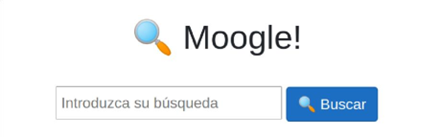
\includegraphics[width=15cm, height=5cm]{img1.png}
		\end{center}
	\end{figure}

\end{center}

\begin{figure}[b]
	\begin{flushleft}
			\textbf{\LARGE{Autor:} \Large{Joel Aparicio Tamayo}}


			\ 


			\textbf{\LARGE{Grupo:} \Large{C-121}}
	\end{flushleft}
\end{figure}



\newpage

\begin{center}
	\textbf{{\Huge {Moogle !}}}
\end{center}


\ 


\begin{center}
	\large\textbf{Especificaciones y particularidades:}
\end{center}


1. El proyecto ha sido probado con un repositorio de alrededor de 15 mil documentos cuyo peso
era de 170 MB (En GitHub estará subida la carpeta Content con solo 10 documentos). Con
estos documentos el proyecto demora alrededor de 1 minuto inicialmente para cargar (solo la
primera vez, luego si se cierra y se abre nuevamente, demora tan solo 10 segundos), y la
búsqueda es casi instantánea.

2. La búsqueda muestra los 10 primeros resultados como máximo. (Pudieran ser más si hay
scores repetidos)

3. El buscador funciona tanto al seleccionar el botón “Buscar”, como al presionar la tecla “Enter”.

4. El snippet mostrado en pantalla de cada documento muestra una vecindad de la primera
aparición de la palabra de más peso de la query con respecto a dicho documento.

5. Se ha implementado el operador de relevancia ($\ast$), el operador de obligatoriedad ({\tiny $\land $}), el
operador de inexistencia (!) y el operador de cercanía ($\sim $). (Dicho funcionamiento será
explicado en la sección “Estructura de Clases \ Operators”)

6. Los operadores {\tiny $\land $} y {!} funcionan solo para la primera palabra de la query que los tenga. (Ej:
“!hola {!}Claudia” solo funcionará para “hola”, mientras que a “Claudia” la tratará como una palabra
normal)

7. Pueden existir combinaciones de los operadores. (Uno en cada palabra distinta, no puede
haber dos juntos en una misma palabra)

8. El operador de cercanía se debe usar de la forma: palabra1 ($\sim $) palabra2 (espacio entre el
operador y las palabras).

\begin{center}
	\large\textbf{Estructura del Proyecto (Dentro de la carpeta Moogle Engine):}
\end{center}


El proyecto posee 8 clases. De ellas hay dos que ya estaban creadas y que no fueron modificadas,
que son: SearchItem y Searchresult. Por tanto, no concierne explicar su funcionamiento en este
informe. Tampoco nos interesa demasiado aquí el funcionamiento de la clase {\textit{Matriz}}, ya que no tiene
aplicación alguna en el buscador (es solo para la parte de Álgebra I). No obstante, esta clase está
bien comentada en el código. Las clases que nos importa explicar son:


\


• \textbf{Repository:} Es la clase que genera el repositorio de documentos. (Ver sección {\textit{“Estrsuctura de Clases”}})

• \textbf{Document:} Es la clase que tiene los métodos para trabajar con los documentos. (Ver sección
{\textit{“Estrsuctura de Clases”}})

• \textbf{RankingVector:} Es la clase que contiene el método para asignarle un score a cada
documento. (Ver sección {\textit{“Estrsuctura de Clases”}})

• \textbf{Operators:} Es la clase que tiene los métodos de los operadores implementados. (Ver sección
{\textit{“Estrsuctura de Clases”}})

• \textbf{Moogle:} Es la clase principal del proyecto y donde se generan los resultados de las
búsquedas. (Ver sección {\textit{“Funcionamiento en tiempo de búsqueda”}})


\ 


\begin{center}
	\large\textbf{Estructura de Clases:}
\end{center}


• \textbf{Repository:}


\


Esta clase estática, como su nombre indica, carga el repositorio, y guarda los datos necesarios
en sus campos estáticos. Los más fundamentales son el campo {\texttt{wordsFrequency}} (una lista de
diccionarios que tendrán como claves cada palabra del documento i, y como valor su TF) y
{\texttt{docsFrequency}} (un diccionario con todas las palabras del corpus como keys, y como valor la
cantidad de documentos en que aparecen).


Además, esta clase tiene el método {\texttt{CreateRepository}} que recibe como parámetro un string
predefinido como “Content”, que es la carpeta donde están los documentos del repositorio. (En
caso de querer cambiar el repositorio de lugar debe pasarse el nombre de dicha carpeta al
método) Este método es el encargado de guardar la información necesaria en los campos
apreciados anteriormente, para ser utilizadas por otras clases. Pero, ¿cómo funciona? A
continuación, se explica brevemente.


Primero almacena las rutas de los documentos en su campo, e inicializa los demás campos.
(En la declaración de los campos se inicializaron con longitud 1 para evitar advertencias por
posibles valores null)


Luego, por medio de un primer bucle for, va a iterar sobre cada documento. Como primera
parte de este bucle, se va a guardar el nombre del documento correspondiente en su campo,
se agregará el texto al campo correspondiente y se le hará Split al texto normalizado (utilizando
el método {\texttt{Normalize}} de la clase {\textit{Document}} -Ver {\textit{Estructura de Clases.Document}} posteriormente-) al texto
para separarlo por palabras (y se eliminarán las cadenas vacías también con
{\texttt{StringSplitOptions.RemoveEmptyEntries}}) y guardarlo en otro campo. Como segunda parte de
este bucle, se itera en un segundo for (esta vez utilizamos foreach) para recorrer cada palabra
del texto (ya que tenemos las palabras separadas ya en uno de los campos). Este bucle interno
va a permitir tener almacenado en otro campo la cantidad de veces que se repite cada palabra
en el documento, y a la vez, en otro campo, en cuántos documentos han ido apareciendo
dichas palabras. A continuación, se aprecia visualmente cómo funciona dicho bucle interno:


\

\begin{figure}[h]
	\begin{center}
		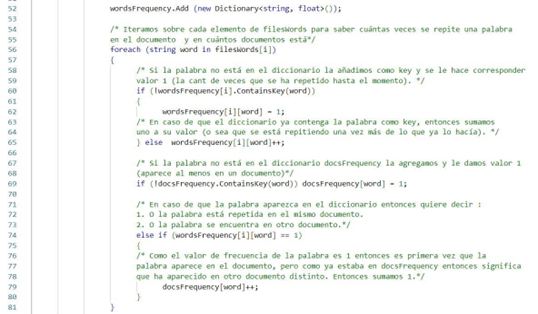
\includegraphics[width = 14cm, height = 9cm]{img2.png}
	\end{center}
\end{figure}

\


Como tercera parte del bucle for externo, y una vez conlcuido el segundo for (foreach), existe
un nuevo for (otro foreach), que itera sobre las palabras sin repetir de cada texto (que en este
caso son las llaves de un diccionario y tienen como valor la cantidad de veces que se repiten)
y teniendo la cantidad de veces que se repiten, se intercambia ese valor (en su diccionario
correspondiente) por su TF (utilizando el método TF de la clase {\textit{Document}} –Ver
{\textit{Estructura de Clases.Document}} posteriormente-). Y de esta manera ya el for externo está completo en su
funcionalidad, y con él, el método también concluye. Una vez que el método es llamado, ya se
podrá obtener la información de los documentos llamando a los campos estáticos de esta clase.
Aclaración: La clase {\textit{Repository}} es estática para que al ser llamado su método en otra parte
puedan ser llenados sus campos sin necesidad de tener que crear un objeto. Esto será
profundizado en la pequeña sección {\textit{“¿Cómo cargar el repositorio?”}}.


\


• \textbf{Document:}


\


Esta clase tiene varias funcionalidades, pero todas relacionadas al trabajo con los documentos
o las palabras de los documentos. Está constituida por 4 métodos: {\texttt{Normalize, NormalizeQuery,
TF, IDF, GetSnippet}}.

El método {\texttt{Normalize}} tiene la función de normalizar un string. Primero lo convierte a minúsculas
y elimina las tildes.En una segunda parte se utiliza el método Replace de la clase {\textit{Regex}} de
{\textit{System.Text.RegularExpressions}} para convertir en espacios en blanco los caracteres
innecesarios. A continuación, se muestra cómo funciona:


\


\begin{figure}[h]
	\begin{center}
		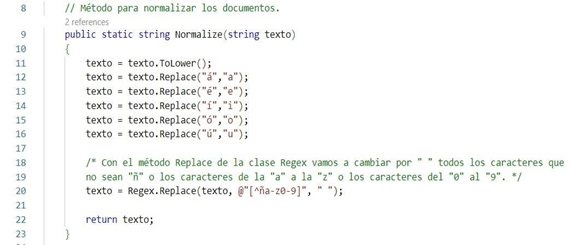
\includegraphics[width = 12cm, height = 5cm]{img3.png}
	\end{center}
\end{figure}


\


Finalmente, el método devuelve el string normalizado.


\


El método {\texttt{NormalizeQuery}} funciona análogamente al método anterior, la única diferencia es
que se mantienen los operadores si los tiene.


El método {\texttt{TF}} recibe dos parámetros: la frecuencia de la palabra en un documento y la cantidad
de palabras de ese documento. Con estos datos devuelve entonces el TF de la palabra que no
es más que el peso de la misma en el documento, y tiene su fórmula específica.
El método {\texttt{IDF}} recibe dos parámetros: la cantidad de documentos y la cantidad de documentos
que poseen la palabra. Con estos datos devuelve entonces el IDF de la palabra que no es más
que el peso de la misma en el cuerpo de documentos, y tiene su fórmula específica.
Por último, se encuentra el método {\texttt{GetSnippet}} que es el que va a generar el snippet a mostrar
en pantalla de cada documento. Recibe como parámetro el índice de un documento.
Primeramente, dentro de un bucle while (true) se guarda el índice de la palabra de la query con
mayor IDF (utilizando los valores almacenados en el campo {\texttt{wordsIDF}} de la clase
{\textit{RankingVector}} –Ver {\textit{Estructura de Clases.RankingVector}} posteriormente-) en la variable {\texttt{index1}}. Luego se
utiliza este índice para obtener la palabra de la query y buscarla en el documento normalizado.
(que estará guardado en la variable {\texttt{text}}). Si el índice es válido y la palabra está en el
documento, pues se rompe el bucle, sino continúa con la siguiente palabra de mayor IDF:


\


\begin{figure}[h]
	\begin{center}
		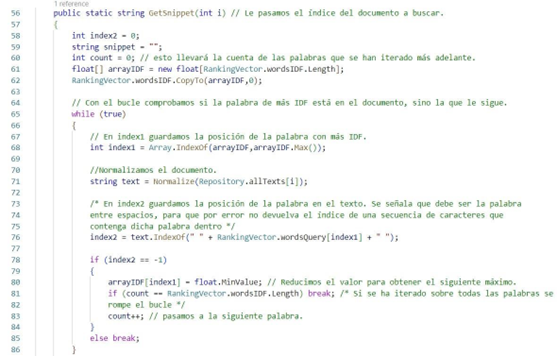
\includegraphics[width = 13cm, height = 8cm]{img4.png}
	\end{center}
\end{figure}


\


Luego de este bucle, el método procede a retornar el snippet dependiendo de si cumple
o no ciertas condiciones:


\ 


\begin{figure}[h]
	\begin{center}
		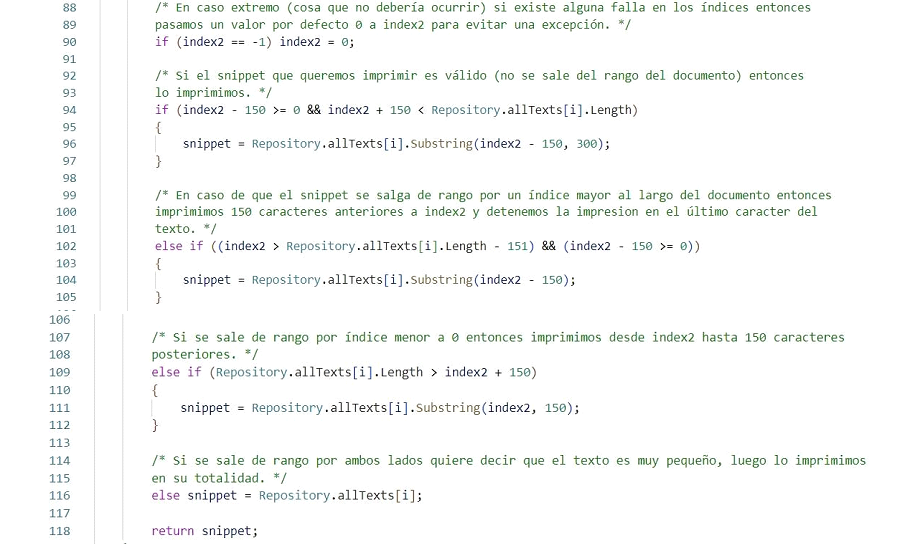
\includegraphics[width = 14cm, height = 9cm]{img5.png}
	\end{center}
\end{figure}


\


• \textbf{RankingVector:}


\


Esta clase está creada para confeccionar el score de los documentos. Posee dos campos
estáticos, uno para guardar la query separada por palabras y poderla utilizar en la clase
{\textit{Document}} para crear el snippet; y otro para almacenar los IDF de cada palabra de la query y
también utilizarlo para crear el snippet.

La clase posee un método llamado {\texttt{GetScore}} que recibe un array con la query separada por
palabras para pasárselo al campo correspondiente en esta clase, un array con los IDF de las
palabras de la query también para pasárselo al campo correspondiente, y el array con los
valores de cercanía. Primeramente, inicializamos algunas variables que serán necesarias
como, por ejemplo, el array final que se va a devolver y una variable que va a ir almacenando
por iteraciones la suma acumulada de TF x IDF.Luego con un bucle for más externo iteramos
sobre la cantidad de documentos. Dentro de este utilizamos un for (foreach) interno para iterar
por las palabras de la query. Utilizando condicionales verificamos si la palabra está en cada
documento. Si está, entonces añadimos a {\texttt{suma}} (inicializada en cero) la multiplicación del TF
de la palabra en ese documento por su IDF.En caso de que la palabra no esté en el documento,
entonces restamos 10 veces la longitud de la query, a {\textit{suma}}, para asegurar que los
documentos que contengan más palabras de la query tengan mayor score. De esta manera,
por ejemplo, si la query contiene 3 palabras y un documento tiene un score de -90, significa
que no contiene ninguna palabra. (Se ha restado 3 veces –una por palabra- la longitud de la
query multiplicada por 10) Así, cuando termine de iterar por las palabras de la query dividimos
la suma entre el valor de cercanía (que será automáticamente 1 si el operador no está, o si una
de las dos palabras no están en el documento) y copiamos el resultado en la posición i del
array final y volvemos a hacer cero la variable {\textit{suma}} para iterar sobre un nuevo documento
en el bucle externo.


\


• \textbf{Operators:}

\


Esta clase contiene los métodos para que la búsqueda admita operadores. Todos los métodos
reciben la query separada por palabras, pero sin normalizar.


Tiene un primer método {\texttt{ItHasToBeInText}} que devuelve el índice de la palabra en al array de
palabras de la query que contenga {\tiny $\land $} (hacer constar que el método trabaja sobre el hecho de
que sea una sola palabra la que empiece con {\tiny $\land $}, en otro caso funcionará, pero solo
correctamente para la primera palabra que contenga {\tiny $\land $}). Para ello, inicializamos una variable
con valor -1 que será la que vamos a devolver. Iteramos sobre las palabras de la query y si una
palabra empieza con {\tiny $\land $}, entonces copiamos su índice en la variable y termina la iteración. (Si
la query tiene la palabra con {\tiny $\land $} pero también la tiene sin el operador, el código también funciona,
pues reconoce que son la misma palabra) Por tanto, el método devolvería -1 si ninguna palabra
posee el operador. Si se usa el operador de cercanía el método analiza si es necesario variar
el índice de la palabra con el operador {\tiny $\land $}.


El segundo método es {\texttt{ItCantBeInText}}, que funcionará análogamente al método anterior lo que
sobre el operador {!}.


El tercer método es {\texttt{ValueOfRelevance}}, que devolverá un diccionario con cada palabra de la
query asociada a su valor. Inicialmente cada valor será 1 (excepto la palabra con el operador
!, pues en este caso la palabra no debe influir en los rankings), pero por medio de una iteración
sobre las palabras de la query y una más interna sobre los caracteres de la palabra (si empieza
con {*}. Si no, saltamos a la siguiente palabra), entonces multiplicamos por 10 ese valor por cada
{*} que tenga la palabra delante.


El cuarto método es {\texttt{Closeness}} que devuelve en un array la cercanía de las dos palabras en cada texto si está
el operador. Si no está, copia 1 a cada elemento del array.


\


\begin{center}
	\large\textbf{¿Cómo cargar el repositorio?}
\end{center}

\


La carga del repositorio de documentos tiene un funcionamiento bastante sencillo. Solamente se llama
al método {\texttt{CreateRepository}} de la clase {\textit{Repository}} en la línea anterior a la que ejecuta la aplicación
en el archivo {\textit{Program}} de la carpeta {\textit{Moogle Server}}:


\


\begin{figure}[h]
	\begin{center}
		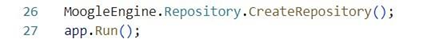
\includegraphics{img6.png}
	\end{center}
\end{figure}


\


En este llamado al método, se llenan los campos de la clase {\textit{Repository}} y se puede usar su
información en las otras clases. Si esta clase no fuera estática habría que crear un objeto en vez de
llamar a la función y entonces los campos quedarían guardando la información de ese objeto y no
habría forma de llamarlos en otras clases fuera de {\textit{Moogle Server}}.


\


\begin{center}
	\large\textbf{Funcionamiento en tiempo de búsqueda:}
\end{center}


\


El funcionamiento en tiempo de búsqueda del programa está regido por la clase {\textit{Moogle}}. En esta
clase se recibe la query como parámetro del método {\texttt{Query}} y se trabaja con ella.


Primeramente, creamos dos arrays donde vamos a guardar la query separada por palabras. En el
primero las guardamos normalizadas manteniendo los operadores (solo lo utilizaremos para los
operadores) y nos aseguramos de no tener palabras repetidas; y en el segundo las guardamos ya
normalizadas. Guardamos además en variables auxiliares ({\texttt{ObligatoryWordIndex}} ({\tiny $\land $}),
{\texttt{NotContainsWordIndex}} ({!}), {\texttt{RelevanceValues}} ({*}), {\texttt{ClosenessValues}} ($\sim $)) los valores que resultan
de evaluar cada método de la clase {\textit{Operators}}. También creamos un array para guardar los valores
de IDF de cada palabra de la query, un diccionario para relacionar más adelante los scores con el
documento correspondiente, un diccionario para relacionar cada palabra de la query y la cantidad de
veces que se repite en la misma, y también el array {\texttt{wordsQuery}}, con las palabras de la query
normalizadas, pero sin repetir. Luego con un foreach llenamos el diccionario poniendo cuántas veces
se repite cada palabra en la query.


En un segundo momento, se crea un primer bucle for para calcular los IDF de las palabras de la query.
Para ello se utiliza una condicional, de manera que, si la palabra está en algún documento, entonces
calculamos su IDF y lo multiplicamos por su valor de relevancia (dado por el operador {*}) y también
por la cantidad de veces que está la palabra en la query. En caso contrario pues mantenemos el cero.


Luego de tener los valores de cada palabra de la query, entonces se crea un array {\texttt{score}} donde se
va a guardar el ranking de los documentos utilizando el método {\texttt{GetScore}} de la clase {\textit{RankingVector}}.
Después, con un pequeño bucle for, le asociamos a cada valor almacenado en {\texttt{score}} el documento
asociado a él (puede haber varios con un mismo valor de score, por eso el diccionario recibe como
valor una lista). Luego ordenamos el ranking de mayor a menor.


Una vez ordenado el ranking, entonces se crea una lista de objetos {\textit{SearchItem}} (título, snippet, score)
que representan cada documento a mostrar en pantalla. Luego existe una condición por si no existen
resultados de búsqueda:


\

\begin{figure}[h]
	\begin{center}
		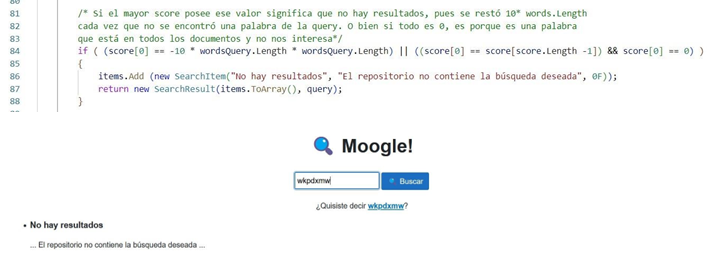
\includegraphics{img7.png}
	\end{center}
\end{figure}


\


En caso de que sí existan resultados, entonces eliminamos primero los valores repetidos en {\texttt{score}}
(pues no son necesarios, ya que si existen repetidos ya uno solo está asociado a una lista con todos
los documentos que poseen dicho ranking), y luego se procede a colocar los diez documentos con
más coincidencias con la búsqueda realizada por el usuario, en la lista mencionada en el párrafo
anterior. Esto se muestra a continuación:


\


\ 


\ 


\ 


\begin{figure}[h]
	\begin{center}
		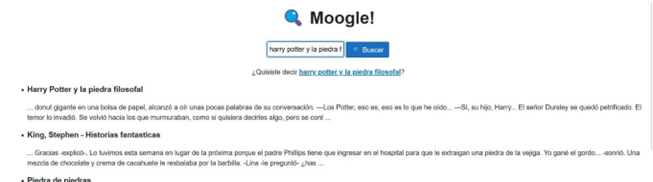
\includegraphics[width = 17cm, height = 5.5cm]{img8.png}
	\end{center}
\end{figure}


\newpage

\begin{figure}[t]
	\begin{center}
		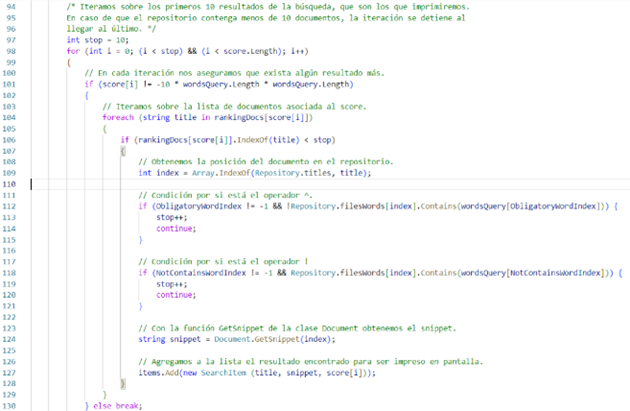
\includegraphics[width = 14cm, height = 10cm]{img9.png}
	\end{center}
\end{figure}


\ 


Para finalizar, nos aseguramos de que la lista de objetos {\textit{SearchItem}} contenga al menos 1. Si es así
pues ya termina prácticamente el método. En caso contrario, se le añade lo siguiente y se muestra
en pantalla:


\


\begin{figure}[h]
	\begin{center}
		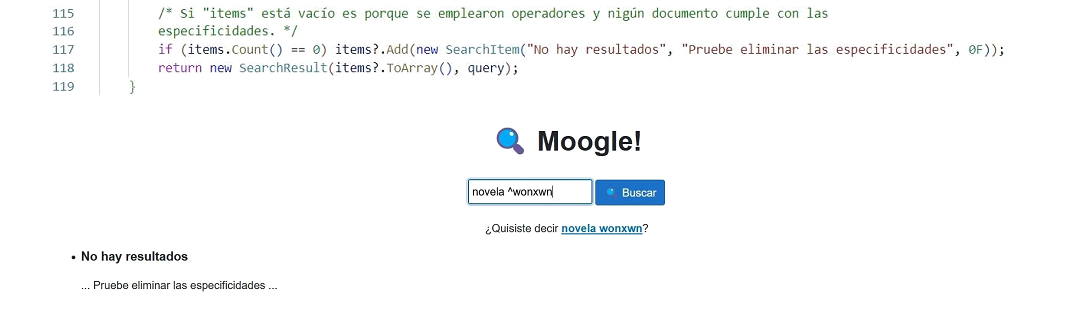
\includegraphics[width=16cm, height=5.5cm]{img10.png}
	\end{center}
\end{figure}

\end{document}